\documentclass[border=4pt]{standalone}
\usepackage{tikz}
\usepackage{amsmath,amssymb}
\usepackage{mathptmx}
\usetikzlibrary{arrows.meta,positioning,calc,shapes.geometric,decorations.pathreplacing,shadows,fadings,patterns}
\definecolor{cblue}{HTML}{1F4E9C}
\definecolor{cgold}{HTML}{D08C00}
\definecolor{cred}{HTML}{B5172E}
\definecolor{cgreen}{HTML}{1B7A3A}
\definecolor{cgrey}{HTML}{555555}
\definecolor{cpurple}{HTML}{5B2A86}
% oblique 3D cuboid: \cuboid{x}{y}{z}{dx}{dy}{dz}{colour}
\newcommand{\cuboid}[7]{%
  \fill[#7!55!white,draw=#7!60!black,line width=0.4pt] (#1,#2,#3+#6) -- ++(#4,0,0) -- ++(0,#5,0) -- ++(-#4,0,0) -- cycle;
  \fill[#7!80!black,draw=#7!60!black,line width=0.4pt] (#1+#4,#2,#3) -- ++(0,#5,0) -- ++(0,0,#6) -- ++(0,-#5,0) -- cycle;
  \fill[#7,draw=#7!60!black,line width=0.4pt] (#1,#2,#3) -- ++(#4,0,0) -- ++(0,0,#6) -- ++(-#4,0,0) -- cycle;}

\usepackage{graphicx}
\begin{document}
\begin{tikzpicture}[x={(1cm,0cm)},y={(0.4cm,0.3cm)},z={(0cm,1cm)},
  arr/.style={-{Stealth[length=2.0mm]},line width=0.6pt},
  lab/.style={font=\footnotesize,align=center},
  note/.style={circle,draw=cpurple!70!black,fill=cpurple!25,inner sep=0pt,minimum size=2.6mm}]
\node[font=\small\bfseries,anchor=west] at (-0.5,0,6.55) {(a) coordinator, subagents, cascade, memory};
% coordinator
\cuboid{-0.3}{0}{2.35}{0.9}{0.9}{0.9}{cblue}
\node[lab,white,font=\scriptsize\bfseries] at (0.15,0,2.8) {coord.};
\node[lab] at (0.15,0,1.95) {budget $\theta$};
% six subagents
\foreach \k/\name in {0/blow-up,1/bypass,2/trivialization,3/residual,4/strong then weak,5/construction}{
  \pgfmathsetmacro\zz{0.2+0.95*\k}
  \cuboid{2.0}{0}{\zz}{0.5}{0.5}{0.5}{cgreen}
  \node[lab,anchor=west,font=\scriptsize,inner sep=1.5pt] (s\k) at (2.78,0,\zz+0.25) {\name};
  \draw[arr,cblue!70!black] (0.65,0,2.8) -- (1.95,0,\zz+0.25);
}
\node[lab,cblue!70!black,fill=white,inner sep=1pt] at (1.25,0,4.25) {$\theta P_{k}$};
% weak checks
\foreach \j in {0,1,2}{\cuboid{5.05+0.5*\j}{0.05}{2.6}{0.35}{0.35}{0.35}{cgold}}
\node[lab] at (5.75,0,3.35) {weak runs $\times r$};
\node[lab,font=\scriptsize] at (5.75,0,2.25) {cost $b$, soundness $\varepsilon$};
\draw[cgrey,line width=0.6pt] (4.6,0,0.45) -- (4.6,0,5.2);
\foreach \k in {0,1,2,3,4,5}{\draw[cgrey,line width=0.4pt] (s\k.east) -- (s\k.east -| 4.6,0);}
\draw[arr,cgrey] (4.6,0,2.77) -- (5.0,0.05,2.77);
% strong check
\cuboid{7.0}{0}{2.45}{0.7}{0.7}{0.7}{cred}
\node[lab,white,font=\scriptsize\bfseries] at (7.35,0,2.8) {exact};
\node[lab] at (7.4,0,3.98) {strong check};
\node[lab,font=\scriptsize] at (7.4,0,3.62) {Lean kernel, cost $c$};
\draw[arr,cgreen] (6.55,0.05,2.77) -- (6.95,0,2.77);
% rejections
\draw[arr,cgrey] (5.75,0.05,2.55) -- (5.75,0,1.25);
\draw[arr,cgrey] (7.35,0,2.4) -- (7.35,0,1.25);
\node[lab,cgrey,draw=gray!50,rounded corners=2pt,fill=white] at (6.55,0,0.85) {rejected: residues recorded};
% memory vault
\begin{scope}[shift={(8.85,0,1.9)}]
  \node[note] (n1) at (0.2,0,1.6) {};
  \node[note] (n2) at (0.9,0,2.1) {};
  \node[note] (n3) at (1.3,0,1.3) {};
  \node[note] (n4) at (0.6,0,0.75) {};
  \node[note] (n5) at (1.45,0,0.35) {};
  \node[note] (n6) at (0.15,0,0.2) {};
  \foreach \a/\b in {n1/n2,n2/n3,n1/n4,n3/n4,n4/n5,n3/n5,n4/n6,n1/n3}{\draw[cpurple!70!black,line width=0.4pt] (\a)--(\b);}
  \node[lab] at (0.8,0,2.75) {linked notes};
\end{scope}
\draw[arr,cgreen] (7.75,0,2.8) -- (8.95,0,3.25) node[pos=0.45,above,lab,cgreen,font=\scriptsize] {kept};
\draw[arr,cpurple!80!black,dashed] (9.0,0,1.95) .. controls (8.6,0,-0.55) and (4.0,0,-0.6) .. (s1.south);
\node[lab,cpurple!80!black,font=\scriptsize] at (9.55,0,1.3) {reuse};
\node[lab,anchor=west,draw=gray!50,fill=white,rounded corners=2pt] at (5.0,0,5.45)
 {$E(r)=br+c(1-\rho)+c\rho\,\varepsilon^{r}$\\[2pt] the strong check is paid on the correct candidates};
\node[anchor=south west,inner sep=0] at (11.1,0,-0.95) {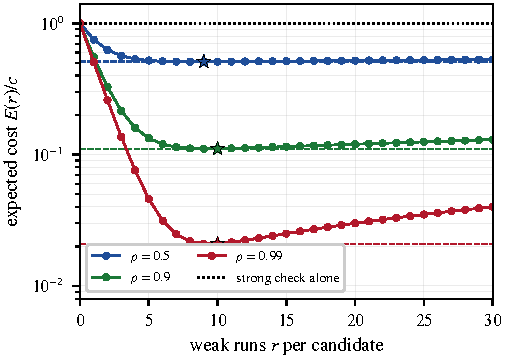
\includegraphics[width=9.0cm]{panel_cascade.pdf}};
\node[font=\small\bfseries,anchor=west] at (11.1,0,6.55) {(b) weak runs before one exact check};
\end{tikzpicture}
\end{document}
